\chapter{Architecture at Hybris}\label{chapter:hybris_architecture}
\section{Overview}\label{section:hybris_architecture/overview}
SAP \acrshort{YaaS} provides a variety of business services to support as well as enhance the products offered as SAP hybris front office such as hybris Commerce, hybris Marketing, hybris Billing etc. Using these offered services, developers can create their own business services focussed on their customer requirements.\\
The figure \ref{fig:hybris_architecture/overview/yaas_overview} provides the overview of \acrshort{YaaS}. \acrshort{YaaS} provides various business processes as a service (bPaaS) essential to develop applications and services thus filling up the gap between SaaS and HCP. For that purpose, it consumes the application services (aPaaS) provided by \acrshort{HCP}.
\begin{figure}[H]
\begin{center}
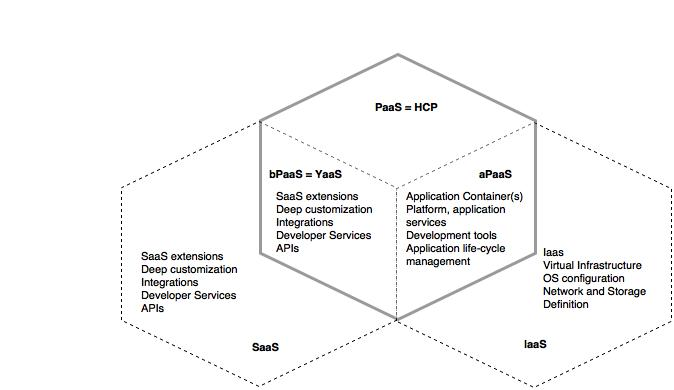
\includegraphics[width=0.8\textwidth]{figures/hybris-architecture-one}
\caption{\acrshort{YaaS} and \acrshort{HCP} \cite{Hirsch:2015aa}}
\label{fig:hybris_architecture/overview/yaas_overview}
\end{center}
\end{figure}
\\
\section{Vision}\label{section:hybris_architecture/vision}
The vision of \acrshort{YaaS} can be clarified with the following statement.
\begin{shaded}
"A cloud platform that allows everyone to easily develop, extend and sell services and applications." \\
\cite{Stubbe:2015aa}
\end{shaded}
The vision can be broadly categorized into following objectives.\\
\begin{enumerate}
\item \textbf{Cloud First}\\
The different parts of the application need to be scaled independently.
\item \textbf{Autonomy}\\
The development teams should be able to develop their modules independent of other teams and able to freely choose the technology that fits the job.
\item \textbf{Retain Speed}\\
The new features will be of value to customers if could be able to be released as fast as possible.
\item \textbf{Community}\\
It should be possible for the components to be shared across internal and external developers.
\end{enumerate}
The definition of microservices \ref{tab:context/microservices_architecture_style/keywords_extracted_from_various_definitions_of_microservice} as well as the characteristics of microservices [ref] signifies clearly that microservices architecture can be a good fit for \acrshort{YaaS} architecture.
\section{YaaS Architecture Principles}\label{section:hybris_architecture/YaaS_architecture_principles}
The Agile Manifesto \cite{Beck:2011aa} provides various principles to develop a software in a better way. It focus on fast response to the requirement changes with frequent continous delivery of software artifacts with close collaboration of customer and self-organizing teams.\\
The Reactive Manifesto \cite{Boner:2014aa} lists various qualities of a reactive system which includes responsiveness (acceptable consistent response time, quick detection and solution of problem), resilience (responsive during the event of failure) , elasticity (responsive during varying amount of workload) and asynchronous message passing. Loose coupling is highly focused.\\
Furthermore, the twelve factors from Heroku \cite{Wiggins:2012aa} provides a methodology for minimizing time and cost to develop software applications as services. It emphasizes on scalability of applications, explicit declaration as well as isolation of dependencies among components, multiple continuous deployments from a single version controlled codebase with separate pipelines for build, release and run.\\
Finally, the microservices architecture provides techiques of developing an application as a collection of autonomous small sized services focused on single responsibility. [section \ref{section:context/microservices_architecture_style}] It focus on independent deployment capability of individual microservices and suggest to use lightweight mechanisms such as http for communication among services. The architecture offers various advantages, few of them being individual independent scalability of each microservice, resilience achieved by isolating failure in a component and technology heterogeneity among various development teams.\cite{Newman:2015aa}
\\
Following the principles mentioned above, a list of principles are compiled to be used as guidelines for creating microservices. \cite{Stubbe:2015aa} The list of principles are listed below.
\\
\textbf{\underline{the y-Factors}}
\\
\begin{enumerate}
\item \textbf{Self-Sufficient Teams}\\
The teams have independence and freedom for any decision related to the design and development of their components. This freedom is balanced by the responsibility for the team to handle the complete lifecycle of their components including smooth running as well as performance in production and troubleshooting in case of any problems.
\item \textbf{Open Technology landscape}\\
The team have freedom to choose any technology that they believe fits the requirement. They are completely responsible for the quality of their product. This gives teams, ownership as well as satisfaction for their products.
\item \textbf{Release early, release often}\\
The agile manifesto and twelve factors from Heroku also focus on continuous delivery of product to the clients. This will decrease time of feedback and ultimately fast response to the feedback resulting in high customer satisfaction. The teams are responsible to create build and delivery pipeline for all available environments.
\item \textbf{Responsibility}\\
The teams are the only responsible groups to work directly with the customers on behalf of their products. They need to work on the feedback provided by the customers. It will increase the quality of the products and relationship with customers. All the responsibilities including scaling, maintaining, supporting and improving products are handled by respective teams.
\item \textbf{\acrshort{API}s first}\\
The \acrshort{API} is a contract between service and consumers. The decision regarding design and development is very important as it can be one of the greatest assets if good or else can be a huge liability if done bad. \cite{Bloch:2016aa} The articles \cite{Bloch:2016aa} and \cite{Blanchette:2008aa} list various characteristics of good \acrshort{API} including simplicity, extensibility, maintainability, completeness, small and focussing on single functionality. Furthermore, a good approach to develop \acrshort{API} is to first design iteratively before implementation in order to understand the requirement clearly. Another important aspect of a good \acrshort{API} among many is complete and updated documentation.
\item \textbf{Predictable and easy-to-use UI}\\
The user interfaces should be simple, consistent across the system and also consistent to various user friendly patterns.\cite{Sollenberger:2012aa} The articles \cite{Martin:2013aa} and \cite{Porter:2016aa} specify additional principles to be considered when designing user interfaces. A few of them includes providing clarity with regard to purpose, smart organization and respecting the expectation as well as requirements of customers.
\item \textbf{Small and Simple Services}
A service should be small and focused on cohesive functionalities. The concept closely relates to the single responsibility principle. \cite{Martin:2016aa} A good approach is to explicitly create boundaries around business capabilities.\cite{Newman:2015aa}
\item \textbf{Scalability of technology}\\
The choice of technologies should be cloud friendly such that the products can scale cost-efficiently and without delay. It is influenced by the elasticity principle provided by the reactive manifesto.\cite{Boner:2014aa}
\item \textbf{Design for failure}
The service should be responsive in the time of failure. It can be possible by containment and isolation of failure within each component. Similarly, the recovery should be handled gracefully without affecting the overal availability of the entire system. \cite{Boner:2014aa}
\item \textbf{Independent Services}\\
The services should be autonomous. Each service should be able to be deployed independently. The services should be loosely coupled, they could be changed independently of eachother. The concept is highly enforced by exposing functionalities via \acrshort{API}s and using lightweight network calls as only way of communication among services. \cite{Newman:2015aa}
\item \textbf{Understand Your System}
It is crucial to have a good understanding of problem domain in order to create a good design. The concept of domain driven design strongly motivates this approach to indentify individual autonomous components, their boundaries and the communication patterns among them. \cite{Newman:2015aa} Furthermore, it is also important to understand the expectations of consumers regarding performance and then to realize them accordingly. It is possible only by installing necessary operational capabilities such as continuous delivery, monitoring, scaling and resilience.
\end{enumerate}
 \section{Modeling Microservices at Hybris}\label{section:hybris_architecture/interview}
 With the intension to anticipate the overall belief, culture and practice followed by hybris to develop \acrshort{YaaS}, a number of interviews were conducted with a subset of key personnels who are directly involved in \acrshort{YaaS}. The list of interviewees with their corresponsing roles is shown in the table \ref{tab:hybris_architecture/interview/interviewee_list}. In order to preserve anonymity, the real names are replaced with forged ones.
\begin{table}[H]
  \centering
  \begin{adjustbox}{max width=\textwidth}
  \begin{tabular}{*{14}{|c}|}%%{|c|l|}
  \hline
\textbf{Names}          & \textbf{Roles}\\      \hline
John Doe                & Product Manager\\     \hline
Ivan Horvat             & Senior Developer\\    \hline
Jane Doe                & Product Manager\\     \hline
Mario Rossi             & Product Manager\\     \hline
Nanashi No Gombe        & Product Manager\\     \hline
Hans Meier              & Architect\\           \hline
Otto Normalverbraucher  & Product Manager\\     \hline
Jan Kowalski            & Senior Developer\\    \hline
\end{tabular}
\end{adjustbox}
  \caption{Interviewee List}
  \label{tab:hybris_architecture/interview/interviewee_list}
\end{table}
\\
\subsection{Hypothesis}\label{section:hybris_architecture/interview/hypothesis}
During the process of solving the concerned research questions, various topics of high value have been discovered. The topics are:\\
\begin{enumerate}
\item Granularity
\item Quality Attributes
\item Process to design microservices
\end{enumerate}
\\
Similarly, based on research findings, a list of hypothesis has been made with respect to each topic.

\begin{shaded}
Hypothesis 1:
\end{shaded}\label{section:hybris_architecture/interview/hypothesis_1}
\textbf{The correct size of microservices is determined by: \begin{enumerate}\item Single Responsibility Principle \item Autonomy, and \item Infrastructure Capability \end{enumerate}}
\\
According S.Newman, a good microservices should be small and focus on accomplishing one thing well. Additionally, it could be independently deployed and updated. This strongly suggests the requirement of \acrshort{SRP} and autonomy respectively. \cite{Newman:2015aa} Futhermore, M. Stine also agree that the size of a microservices should be determined by single responsibility principle. \cite{Stine:2014aa}
Also, the principle listed in \ref{principle:granularity/IT_infrastructure} indicate that the advancement in the current technology and culture of the organization also defines size of microservices. \cite{Pierre-Reldin:2007aa}
\begin{shaded}
Hypothesis 2:
\end{shaded} \label{section:hybris_architecture/interview/hypothesis_2}
\textbf{Domain driven design is the optimum approach to design microservices.}
\\
\\
The concept of domain driven design to design microservices is promoted by S. Newman and M. Fowler. \cite{Newman:2015aa} \cite{Fowler:2014aa} Similary, there can be found evendence of domain driven design being used in various projects to design microservices. The list of projects is shown in the table \ref{tab:domain_driven_design/microservices_and_bounded_context/Microservices_following_Bounded_Context}.
\\
\subsection{Interview Compilation}\label{section:hybris_architecture/interview/interview_compilation}
For each topic listed above in section \ref{section:hybris_architecture/interview/hypothesis}, a list of questionaires is prepared. The questions were then asked to the interviewees. In the remaining part of this section, an attempt is made to compile the response from the interviews on the questionaires for each topic.
\\
\textbf{\underline{1. Granularity}}\\  
\begin{shaded} Question 1.1 \end{shaded} \label{question:hybris_architecture/interview/question_1.1}
"Do you consider the size of microservices when desigining microservice architecture?"\\
\begin{comment}
\begin{table}[H]
\centering
\begin{adjustbox}{max width=\textwidth}
\begin{tabular}{*{14}{|c}|}%%{|c|l|l|l|l|l|l|l|l|l|}
\hline
\textbf{Response 1.1} & John & Ivan & Jane & Mario & Nanashi & Hans & Otto & Jan & \textbf{Score}\\
 \hline
Important               & 1 & 1 & 1 & 0 & 1 & 1 & 0 & 0 & \textbf{5}    \\ 
 \hline
Secondary, Not primary  & 0 & 0 & 0 & 1 & 0 & 0 & 1 & 1 & \textbf{3} \\ 
 \hline
Not Important           & 0 & 0 & 0 & 0 & 0 & 0 & 0 & 0 & \textbf{0} \\ 
 \hline
 \hline
\end{tabular}
\end{adjustbox}
\label{tab:hybris_architecture/interview/question_1.1}
\end{table}
\end{comment}
\\
\\
\begin{comment}
\begin{figure}[H]
\begin{center}
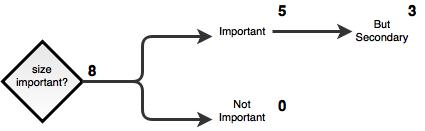
\includegraphics[width=0.9\textwidth]{figures/hybris_architecture_question_1_1}
\label{fig:hybris_architecture/interview/hybris-architecture-question-1-1}
\end{center}
\end{figure}
\\
\end{comment}

\\
\begin{figure}[H]
\begin{center}
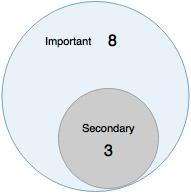
\includegraphics[scale=0.5]{figures/question1_1}
\label{fig:hybris_architecture/interview/question1-1}
\end{center}
\end{figure}
\\

\begin{shaded} Question 1.2 \end{shaded} \label{question:hybris_architecture/interview/question_1.2}
"How do you measure size of a microservice?"\\
\begin{comment}
\begin{table}[H]
\centering
\begin{adjustbox}{max width=\textwidth}
\begin{tabular}{*{14}{|c}|}%%{|c|c|l|l|l|l|l|l|l|l|l|}
\hline
\multicolumn{2}{|c|}{\textbf{Response 1.2} }& John & Ivan & Jane & Mario & Nanashi & Hans & Otto & Jan & \textbf{Score}\\
 \hline
 \hline
\multicolumn{2}{|c|}{\textit{Qualitatively}}               & 1 & 1 & 1 & 1 & 1 & 1 & 1 & 1 & \textbf{8}    \\ 
 \hline
a.& Functionality  & 1 & 1 & 1 & 1 & 1 & 1 & 1 & 1 & \textbf{8}\\ 
 \hline
b.& Business value           & 1 & 1 & 1 & 1 & 1 & 1 & 1 & 1 & \textbf{8} \\ 
 \hline
 \hline
 \multicolumn{2}{|c|}{\textit{Quantitatively}}               & 0 & 0 & 0 & 0 & 0 & 0 & 0 & 0 & \textbf{0}    \\ 
 \hline
 \hline
\end{tabular}
\end{adjustbox}
\label{tab:hybris_architecture/interview/question_1.2}
\end{table}
\end{comment}
\\
\begin{comment}
\\
\begin{figure}[H]
\begin{center}
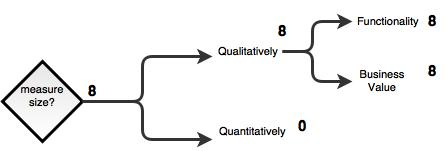
\includegraphics[width=0.9\textwidth]{figures/hybris_architecture_question_1_2}
\label{fig:hybris_architecture/interview/hybris-architecture-question-1-2}
\end{center}
\end{figure}
\\
\end{comment}

\\
\begin{figure}[H]
\begin{center}
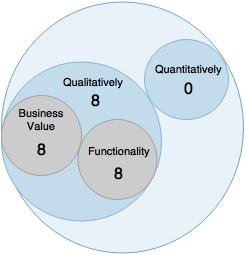
\includegraphics[scale=0.5]{figures/question1_2}
\label{fig:hybris_architecture/interview/question1-2}
\end{center}
\end{figure}
\\

\begin{shaded} Question 1.3 \end{shaded} \label{question:hybris_architecture/interview/question_1.3}
"What kind of size do you try to achieve for a microservice?"\\

\begin{comment}
\begin{table}[H]
\centering
\begin{adjustbox}{max width=\textwidth}
\begin{tabular}{*{14}{|c}|}%%{|c|c|l|l|l|l|l|l|l|l|l|}
\hline
\multicolumn{2}{|c|}{\textbf{Response 1.3} }
                                    & John & Ivan & Jane & Mario & Nanashi & Hans & Otto & Jan & \textbf{Score}\\
 \hline
 \hline
\multicolumn{2}{|c|}{\textit{as small as possible in terms of functionality}}               
                                    & 1 & 1 & 1 & 1 & 1 & 1 & 1 & 1 & \textbf{8}    \\ 
 \hline
 \hline
 \multicolumn{2}{|c|}{\textit{influenced by other attributes}}               
                                    &   &   &   &   &   &   &   &   &     \\ 
 \hline
a.& Business Value                  & 1 & 1 & 1 & 1 & 1 & 1 & 1 & 1 & \textbf{8}\\ 
 \hline
b.& Single Responsibility           & 1 & 1 & 1 & 1 & 1 & 1 & 1 & 1 & \textbf{8} \\ 
 \hline
c.& Loose Coupling                  & 0 & 1 & 0 & 0 & 1 & 1 & 0 & 1 & \textbf{4} \\ 
 \hline
d.& Cohesion                        & 0 & 1 & 0 & 0 & 0 & 0 & 1 & 1 & \textbf{3} \\ 
 \hline
e.& Autonomy                        & 0 & 1 & 1 & 0 & 0 & 1 & 0 & 0 & \textbf{3} \\ 
 \hline
f.& Maintainability                 & 0 & 1 & 0 & 0 & 0 & 1 & 1 & 0 & \textbf{3} \\ 
 \hline
g.& Reusability                     & 0 & 1 & 0 & 0 & 1 & 1 & 1 & 0 & \textbf{4} \\ 
 \hline
h.& Scalability                     & 1 & 1 & 0 & 1 & 1 & 1 & 1 & 0 & \textbf{6} \\ 
 \hline
i.& Network Complexity              & 1 & 0 & 0 & 0 & 1 & 1 & 0 & 0 & \textbf{3} \\ 
 \hline
 \hline
\end{tabular}
\end{adjustbox}
\label{tab:hybris_architecture/interview/question_1.3}
\end{table}
\end{comment}
\\
\begin{comment}
\\
\begin{figure}[H]
\begin{center}
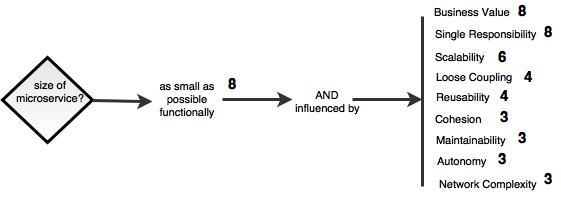
\includegraphics[width=0.9\textwidth]{figures/hybris_architecture_question_1_3}
\label{fig:hybris_architecture/interview/hybris-architecture-question-1-3}
\end{center}
\end{figure}
\\
\end{comment}
\\
\begin{figure}[H]
\begin{center}
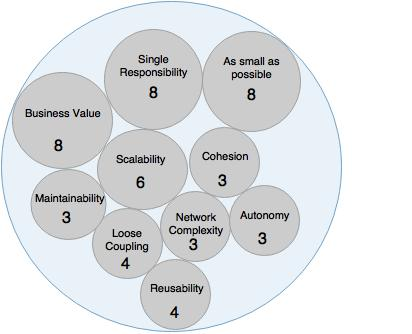
\includegraphics[scale=0.5]{figures/question1_3}
\label{fig:hybris_architecture/interview/question1-3}
\end{center}
\end{figure}
\\
\begin{shaded} Question 1.4 \end{shaded} \label{question:hybris_architecture/interview/question_1.4}
"Suppose that you do not have the agile culture like continuous integration and delivery automation and also cloud infrastructure. How will it affect your decision regarding microservices and their size?"\\
\begin{table}[H]
\centering
\begin{adjustbox}{max width=\textwidth}
\begin{tabular}{*{14}{|c}|}%%{|c|l|l|l|l|l|l|l|l|l|}
\hline
\textbf{Response 1.4}   & John & Ivan & Jane & Mario & Nanashi & Hans & Otto & Jan & \textbf{Score}\\
 \hline
 \begin{tabular}{ll}
                    \multirow{2}{*}
                    & No microservices at all, start with Monolith,\\
                    & extract one microservice at a time as automation matures\\
                    \end{tabular}
               
                                & 1 & 1 & 0 & 1 & 1 & 1 & 1 & 1 & \textbf{7}    \\ 
 \hline
  \begin{tabular}{ll}
                    \multirow{2}{*}
                    & Start with bigger sized microservices with\\
                    & high business value, low coupling and single Responsibility\\
                    \end{tabular}  
                                & 0 & 0 & 1 & 0 & 1 & 0 & 1 & 0 & \textbf{3} \\ 
 \hline
 \hline
\end{tabular}
\end{adjustbox}
\label{tab:hybris_architecture/interview/question_1.4}
\end{table}
\\
\begin{comment}
\\
\begin{figure}[H]
\begin{center}
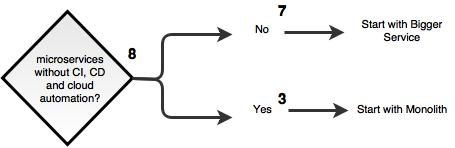
\includegraphics[width=0.9\textwidth]{figures/hybris_architecture_question_1_4}
\label{fig:hybris_architecture/interview/hybris-architecture-question-1-4}
\end{center}
\end{figure}
\\
\\
\begin{figure}[H]
\begin{center}
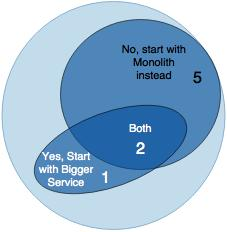
\includegraphics[scale=0.5]{figures/question1_4}
\label{fig:hybris_architecture/interview/question1-4}
\end{center}
\end{figure}
\\
\end{comment}
\begin{shaded} Question 1.5 \end{shaded} \label{question:hybris_architecture/interview/question_1.5}
"Are you facing any complexities because of microservices architecture and the size you have chosen?"\\
\begin{table}[H]
\centering
\begin{adjustbox}{max width=\textwidth}
\begin{tabular}{*{14}{|c}|}%%{|c|l|l|l|l|l|l|l|l|l|}
\hline
\textbf{Response 1.5}   & John & Ivan & Jane & Mario & Nanashi & Hans & Otto & Jan & \textbf{Score}\\
 \hline
communication overhead in network               & 0 & 1 & 0 & 0 & 0 & 0 & 1 & 0 & \textbf{2}    \\ 
 \hline
complexity in failure handling  & 0 & 1 & 0 & 0 & 0 & 0 & 0 & 0 & \textbf{1} \\ 
 \hline
Monitoring is difficult           & 0 & 1 & 0 & 0 & 0 & 0 & 1 & 0 & \textbf{1} \\ 
 \hline
 Operational support is costly           & 0 & 1 & 1 & 0 & 0 & 0 & 0 & 0 & \textbf{2} \\ 
 \hline
 difficult to trace a request           & 0 & 1 & 1 & 0 & 0 & 0 & 0 & 0 & \textbf{2} \\ 
 \hline
 updates can be difficult due to dependencies among microservices          & 0 & 0 & 1 & 0 & 0 & 0 & 0 & 0 & \textbf{1} \\ 
 \hline
 \hline
\end{tabular}
\end{adjustbox}
\label{tab:hybris_architecture/interview/question_1.5}
\end{table}
\\


\textbf{\underline{2. Quality Attributes}}\\
\begin{shaded} Question 2.1 \end{shaded} \label{question:hybris_architecture/interview/question_2.1}
"Do you consider any quality attributes when selecting microservices?"\\
\begin{table}[H]
\centering
\begin{adjustbox}{max width=\textwidth}
\begin{tabular}{*{14}{|c}|}%%{|c|l|l|l|l|l|l|l|l|l|}
\hline
\textbf{Response 2.1}   & John & Ivan & Jane & Mario & Nanashi & Hans & Otto & Jan & \textbf{Score}\\
 \hline
Loose Coupling          & 1 & 1 & 1 & 1 & 1 & 1 & 1 & 1 & \textbf{8}    \\ 
 \hline
Cohesion                & 1 & 1 & 1 & 1 & 1 & 1 & 0 & 1 & \textbf{7}    \\ 
 \hline
 Autonomy               & 1 & 1 & 0 & 0 & 0 & 1 & 1 & 0 & \textbf{4}    \\ 
 \hline
 Scalability            & 1 & 0 & 0 & 1 & 1 & 0 & 1 & 1 & \textbf{5}    \\ 
 \hline
 Complexity             & 1 & 0 & 0 & 0 & 1 & 0 & 1 & 0 & \textbf{3}    \\ 
 \hline
 Reusability            & 0 & 1 & 0 & 0 & 0 & 0 & 1 & 0 & \textbf{2}    \\ 
 \hline
 \hline
\end{tabular}
\end{adjustbox}
\label{tab:hybris_architecture/interview/question_2.1}
\end{table}
\\

\begin{shaded} Question 2.2 \end{shaded} \label{question:hybris_architecture/interview/question_2.2}
"Do you consider any metrics for evaluating the quality attributes?"\\
\begin{comment}
\begin{table}[H]
\centering
\begin{adjustbox}{max width=\textwidth}
\begin{tabular}{*{14}{|c}|}%%{|c|l|l|l|l|l|l|l|l|l|}
\hline
\textbf{Response 2.2}   & John & Ivan & Jane & Mario & Nanashi & Hans & Otto & Jan & \textbf{Score}\\
 \hline
No          & 1 & 1 & 1 & 1 & 1 & 1 & 1 & 1 & \textbf{8}    \\ 
 \hline
Yes                & 0 & 0 & 0 & 0 & 0 & 0 & 0 & 0 & \textbf{0}    \\ 
 \hline
\end{tabular}
\end{adjustbox}
\label{tab:hybris_architecture/interview/question_2.2}
\end{table}
\end{comment}
\\
\begin{comment}
\\
\begin{figure}[H]
\begin{center}
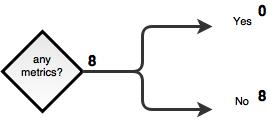
\includegraphics[scale=0.5]{figures/hybris_architecture_question_2_2}
\label{fig:hybris_architecture/interview/hybris-architecture-question-2-2}
\end{center}
\end{figure}
\\
\end{comment}
\\
\begin{figure}[H]
\begin{center}
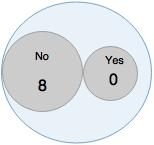
\includegraphics[scale=0.5]{figures/question2_2}
\label{fig:hybris_architecture/interview/question2-2}
\end{center}
\end{figure}
\\
\begin{shaded} Question 2.3 \end{shaded} \label{question:hybris_architecture/interview/question_2.3}
"Do you think the table of basic metrics can be helpful?"\\
\begin{comment}
\begin{table}[H]
\centering
\begin{adjustbox}{max width=\textwidth}
\begin{tabular}{*{14}{|c}|}%%{|c|l|l|l|l|l|l|l|l|l|}
\hline
\textbf{Response 2.3}   & John & Ivan & Jane & Mario & Nanashi & Hans & Otto & Jan & \textbf{Score}\\
 \hline
No          & 0 & 0 & 0 & 0 & 0 & 0 & 0 & 0 & \textbf{0}    \\ 
 \hline
Yes                & 1 & 0 & 1 & 0 & 1 & 0 & 1 & 0 & \textbf{4}    \\ 
 \hline
Maybe                & 0 & 1 & 0 & 1 & 0 & 1 & 0 & 1 & \textbf{4}    \\ 
 \hline
 \hline
\end{tabular}
\end{adjustbox}
\label{tab:hybris_architecture/interview/question_2.3}
\end{table}
\end{comment}
\\
\begin{comment}
\\
\begin{figure}[H]
\begin{center}
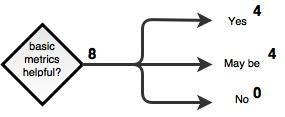
\includegraphics[scale=0.5]{figures/hybris_architecture_question_2_3}
\label{fig:hybris_architecture/interview/hybris-architecture-question-2-3}
\end{center}
\end{figure}
\\
\end{comment}
\\
\begin{figure}[H]
\begin{center}
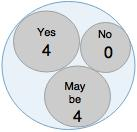
\includegraphics[scale=0.5]{figures/question2_3}
\label{fig:hybris_architecture/interview/question2-3}
\end{center}
\end{figure}
\\
\textbf{\underline{3. Process to design microservices}}\\
\begin{shaded} Question 3.1 \end{shaded} \label{question:hybris_architecture/interview/question_3.1}
"Do you follow specific set of consistent procedures across the teams to discover microservices?"\\
\begin{comment}
\begin{table}[H]
\centering
\begin{adjustbox}{max width=\textwidth}
\begin{tabular}{*{14}{|c}|}%%{|c|l|l|l|l|l|l|l|l|l|}
\hline
\textbf{Response 3.1}   & John & Ivan & Jane & Mario & Nanashi & Hans & Otto & Jan & \textbf{Score}\\
 \hline
No          & 1 & 1 & 1 & 1 & 1 & 1 & 1 & 1 & \textbf{8}    \\ 
 \hline
Yes                & 0 & 0 & 0 & 0 & 0 & 0 & 0 & 0 & \textbf{0}    \\ 
 \hline
\end{tabular}
\end{adjustbox}
\label{tab:hybris_architecture/interview/question_2.3}
\end{table}
\end{comment}
\\
\begin{comment}
\\
\begin{figure}[H]
\begin{center}
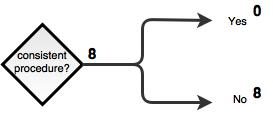
\includegraphics[scale=0.5]{figures/hybris_architecture_question_3_1}
\label{fig:hybris_architecture/interview/hybris-architecture-question-3-1}
\end{center}
\end{figure}
\\
\end{comment}
\\
\begin{figure}[H]
\begin{center}
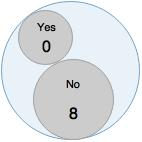
\includegraphics[scale=0.5]{figures/question3_1}
\label{fig:hybris_architecture/interview/question3-1}
\end{center}
\end{figure}
\\
\begin{shaded} Question 3.2 \end{shaded} \label{question:hybris_architecture/interview/question_3.2}
"Can you define the process you follow to come up with microservices?"\\
\begin{comment}
\begin{table}[H]
\centering
\begin{adjustbox}{max width=\textwidth}
\begin{tabular}{*{14}{|c}|}%%{|c|l|l|l|l|l|l|l|l|l|l|}
\hline
\multicolumn{3}{|c|}{\textbf{Response 3.2}}   & John & Ivan & Jane & Mario & Nanashi & Hans & Otto & Jan & \textbf{Score}\\
\hline
\hline
\multicolumn{3}{|c|}{
\begin{tabular}{ll}
\multirow{4}{*}
& By brain-storming to divide a usecase into finer\\
& functionalities considering business value, cohesion,\\
& loose coupling [Single Responsibility], autonomy,\\
& reusability and scalability.
\end{tabular}}
                                            & 1 & 0 & 1 & 1 & 0 & 0 & 1 & 1 & \textbf{5}    \\ 
 \hline
& \multicolumn{2}{|c|}{\textit{Have you heard of Domain driven design and bounded context?}}               
                                            &   &   &   &   &   &   &   &   &      \\ 
 \hline
 & & Yes                                    & 0 &   & 0 & 0 &   &   & 1 & 0 & \textbf{1}    \\ 
 \hline
 & \multicolumn{2}{|c|}{\textit{Is the concept provided by bounded context being used?}}               
                                            &   &   &   &   &   &   &   &   &      \\ 
 \hline
 & & Yes                                    & 1 & 0 & 1 & 0 & 0 & 0 & 1 & 0 & \textbf{3}    \\
 \hline
 \hline
\multicolumn{3}{|c|}{
\begin{tabular}{ll}
\multirow{4}{*}
& By identifying bounded context using domain-driven-design\\
& Understand the problem domain interacting with\\
& domain experts and studying the interaction among\\
& domain models and flow of data.
\end{tabular}}
                                            & 0 & 1 & 0 & 0 & 1 & 1 & 1 & 0 & \textbf{4}    \\ 
\hline
\hline
\end{tabular}
\end{adjustbox}
\label{tab:hybris_architecture/interview/question_3.2}
\end{table}
\end{comment}
\\
\begin{comment}
\\
\begin{figure}[H]
\begin{center}
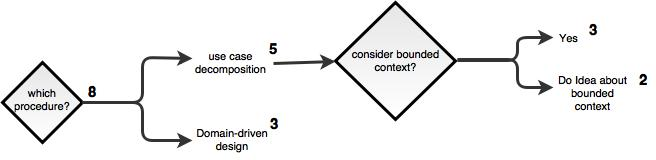
\includegraphics[scale=0.5]{figures/hybris_architecture_question_3_2}
\label{fig:hybris_architecture/interview/hybris-architecture-question-3-2}
\end{center}
\end{figure}
\\
\end{comment}
\\
\begin{figure}[H]
\begin{center}
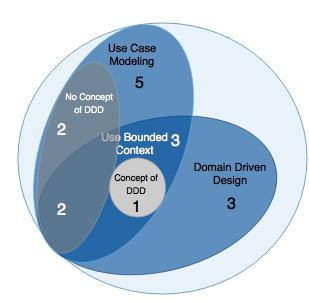
\includegraphics[scale=0.5]{figures/question3_2}
\label{fig:hybris_architecture/interview/question3-2}
\end{center}
\end{figure}
\\
\subsection{Interview Reflection on Hypothesis}\label{section:hybris_architecture/interview/interview_reflection_on_hypothesis}
The data gathered from the interviews which are compiled in the section \ref{section:hybris_architecture/interview/interview_compilation} can be a good source to analyse the hypothesis listed on the section \ref{section:hybris_architecture/interview/hypothesis}.
\\
\begin{shaded} Hypothesis 1 \end{shaded}
\textbf{The correct size of microservices is determined by: \begin{enumerate}\item Single Responsibility Principle \item Autonomy, and \item Infrastructure Capability \end{enumerate}}
\\
The response from question \ref{question:hybris_architecture/interview/question_1.3} has helped to point out some important constraints which play significant role in industry while choosing appropriate size of microservice. It is also interesting to notice how the terms in answer closely relate to the hypothesis \ref{section:hybris_architecture/interview/hypothesis_1}. The figure attempts to clarify the relationship among the terms with the hypothesis.
\\

\\
\begin{figure}[H]
\begin{center}
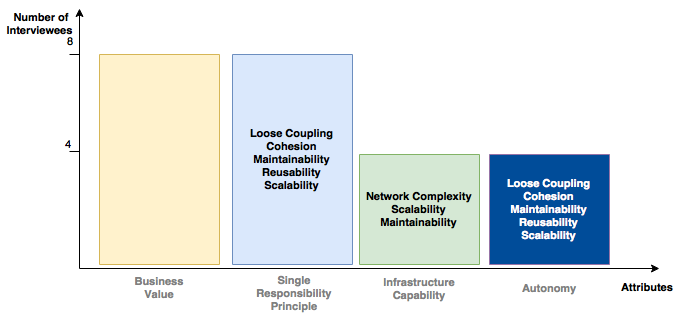
\includegraphics[width=0.8\textwidth]{figures/hybris-architecture-two}
\caption{Attributes grouping from interview response}
\label{fig:hybris_architecture/interview/attributes_grouping}
\end{center}
\end{figure}
\\
The interview unfolded various quality attributes which determine the correct size of a microservice. Moreover, these quality attributes can be classified into three major groups which are: \\
\begin{enumerate}
\item Single Responsibility Principle
\item Automony
\item Infrastructure Capability
\end{enumerate}
\\
Additionally, the response from the question \ref{question:hybris_architecture/interview/question_1.4} highly suggest the significance of availability of proper infrastructure to decide about size of microservices and the microservices architecture.
This highly moves in the direction to support the hypothesis.\\
Finally, there appears one additional constraint to affect the size of microservices, not covered by hypothesis but mentioned by all interviewees, which is the business value provided by the microservices.
\\
\begin{shaded} Hypothesis 2 \end{shaded}
\textbf{Domain driven design is the optimum approach to design microservices.}
\\
From the response to question \ref{question:hybris_architecture/interview/question_3.1}, it can be implied that the organization has no consistent set of specific guidelines which are agreed and pratised across all teams. However,  
the various reactions to the question \ref{question:hybris_architecture/interview/question_3.2} appear to fall with two class of process. The response from \ref{question:hybris_architecture/interview/question_3.2} is repeated here again for convenience \ref{fig:hybris_architecture/interview/process_variations_to_design_microservices}.\\
\\
\begin{figure}[H]
\begin{center}
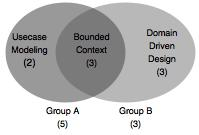
\includegraphics[scale=0.5]{figures/hybris-architecture-three}
\caption{Process variations to design microservices}
\label{fig:hybris_architecture/interview/process_variations_to_design_microservices}
\end{center}
\end{figure}
\\
There is one group of reactions which follow a process to functionally divide a usecase into small functions based upon various factors such as single responsiblity and the requirements of performance. This strongly resemble to the usecase modeling technique as described in the chapter \ref{chapter:selection_by_use_case}. 
\\Moreover, within the same group, a partition are also using the concept of bounded context to ensure autonomy, which also suggests towards the direction of domain driven design as mentioned in the chapter \ref{chapter:domain_driven_design}. It is interesting to find out that some of the teams are using the concept of bounded context implicitly even without its knowledge. The rest of the teams who were not using bounded context, have no idea about the concept. It may be assumed that they will have different view once they get familiar with the concept.
\\
Finally, the rest of the interviewees agree on domain driven design to be the process to design microservices. So, the  response is of mixed nature, both usecase modeling and domain driven design are used in desigining microservices. However, it should also be stated that domain driven design are used on its own or along with usecase modeling to design autonomous microservices.

 \section{Derivation of Modeling Approach at Hybris by interview compilation}\label{section:hybris_architecture/interview_summary}
 The response from the interviews as compiled in section \ref{section:hybris_architecture/interview/interview_compilation} is analyzed for each topic listed in \ref{section:hybris_architecture/interview/hypothesis} separately.
 \\
 \\
 \textbf{Granularity}
 \\
 \\
Granularity of a microservice is considered as an important aspect when designing microservices architecture. The first impression in major cases is to make the size of microservice as small as possible however there are also various attributes and concepts which affects the decision regarding the size of microservices. The major aspects are single responsibility principle, autonomy and infrastructure capability.
\\
The single responsibility gives impression to assume the size of a microservice as small as possible so that the service has minimum cohesive functionality and less number of consumers affected. Whereas, in order to make the microservice autonomous, the service should have full control over its resources and less dependencies upon other services for accomplishing its core logic. This suggests that the size of the service should be big enough to cover the transactional boundary upon its core logic and have full control on its business resources. 
\\
Moreover, the small the size of the service is, the number of required microservices increases to accomplish the functionalities of the application. This increases network complexity. Additionally, the logical complexity as well as maintainability will increase. Undoubtedly, the independent scalability of individual service will also increase. However, this increases the operational complexity for maintaining and deploying the microservices, due to the number of services and number of environment to be maintained for each services.
\\
As shown in \ref{fig:hybris_architecture/interview/attributes_grouping}, various factors affect the size of microservices.
The research findings as well as interview response leads to the idea that the question regarding "size" of a microservices has no straight answer. The answer itself is a multiple objective optimization problem whose answer depend upon the level of abstraction of the problem domain achieved, self-governance requirement, self-containment requirement and the honest capability of the organization to handle the operational complexity.
\\
Finally, there is an additional deciding factor called "Business Value". The chosen size of the microservice should give business and competitive advantage to the organization and closely lean towards the organizational goals. A decision for a group of cohesive functionalities to be assigned as a single microservice means that a dedicated resources in terms of development, scaling, maintainance, deployment and cloud resources have to be assigned. A rational decision would be to relate the expected business value of the microservice against the expected cost value required by it.
\\
\\
\textbf{Quality Attributes}
\\
\\
The teams do not follow any quantitative metrics for measuring various quality attributes. However, they agree on a common list of quality attributes to be considered as shown in the table \ref{tab:hybris_architecture/interview/question_2.1}. According to the reactions from interviews, the basic metrics to evaluate the quality attributes visualized in the table  \ref{tab:quality_of_service/quality_attributes/basic_quality_metrics} can be helpful to approach the design of microservices architecture in an efficient way.
\\
\\
\textbf{Process to design microservices}
\\
\\
There is no single consistent process followed across all the teams. Each team has its own steps to come up with microservices. However, the steps and decision are highly influenced by a set of \abrshort{YaaS} standard principles \ref{section:hybris_architecture/YaaS_architecture_principles}. The reactions from the interviewees are already visualized in \ref{fig:hybris_architecture/interview/process_variations_to_design_microservices}. 
\\
The process followed by a portion of teams closely relate to usecase modeling approach, where a usecase is divided into several smaller abstractions guided by cohesion, reusability and single responsibility principle. Within this group, a major number of teams also use the concept of bounded concept in order to realize autonomous boundary around the service. Finally, the remaining portion of the teams closely follow domain driven design, where a problem domain is divided into sub-domains and in each sub-domain, various bounded contexts are discovered, which is then mapped into microservices. 
\\
The domain driven design can be considerd as the most suitable approach to design microservices. Following this approach, not only the problem domain is functionally divided into cohesive group of functionalities but also leads to a natural boundary around the cohesive functionalities with respect the real world, where concept as well as differences are well understood and the ownership of business resources and core logic are well preserved.

 \section{Example Scenario}\label{section:hybris_architecture/example_scenario}
 \acrshort{YaaS} provides a cloud platform where customers can buy and sell applications and services. In order to accomplish this, \acrshort{YaaS} offers various basic business and core functionalities as microservices. The customers can either use or extend these services to create new services and applications focusing on their individual requirements and goals.
 \\
The following part of this section discuss the steps used to identify the basic microservices in \acrshort{YaaS}.
\\
\textbf{\underline{Step 1:}}
\\
The problem domain is studied thoroughly to identify core domains, supporting domains and generic domains.
\begin{table}[H]
  \centering
  \begin{adjustbox}{max width=\textwidth}
  \begin{tabular}{*{14}{|c}|}%%{|c|c|c|}
  \hline
  \# & \textbf{Sub-domain}  & \textbf{Type} & \textbf{Description}\\
  \hline
  \hline
   1 & Checkout         & Core          & handles overall process from cart creation to selling of cart items.\\ \hline \hline
   2 & Product          & Supporting    & deals with product inventory\\ \hline
   3 & Customer         & Supporting    & deals with customer inventory\\ \hline
   4 & Coupon           & Supporting    & deals with coupon management \\ \hline
   5 & Order            & Supporting    & handles orders management\\ \hline \hline
   6 & Email            & Generic       & provides REST api for sending emails\\ \hline
   7 & Event            & Generic       & provides asynchronous event based notification service\\ \hline
   8 & Account          & Generic       & handles users and roles management\\ \hline
   9 & OAuth2           & Generic       & provides authentication for clients to access resource of resource-owner \\ \hline 
   \hline
   \end{tabular}
\end{adjustbox}
  \caption{Sub-domains in \acrshort{YaaS}}
  \label{tab:hybris_architecture/example_scenario/sub-domains-in-YaaS}
\end{table}
\\
\textbf{\underline{Step 2:}}
\\
The major functionality of the commerce platform is to sell products, which makes 'Checkout' the core sub-domain. The sub-domain is responsible for a bunch of independent responsibilities. The individual independent functionalities can be rightfully represented by respective bounded contexts. The bounded contexts are realized using microservices. The other major reason for them to be made microservices, in addition to single independent responsibility, is different scalability requirements for each functionality.
\begin{table}[H]
  \centering
  \begin{adjustbox}{max width=\textwidth}
  \begin{tabular}{*{14}{|c}|}%%{|c|c|}
  \hline
  \# & \textbf{Bounded Context}  & \textbf{Description}\\
  \hline
  \hline
   1 & Checkout             & handles the orchestration logic for checkout \\ \hline
   2 & Cart                 & handles cart inventory \\ \hline
   3 & Cart Calculation     & calculates net value of cart considering various constraints such as tax, discount etc. 
   \\ \hline
   \hline
   \end{tabular}
\end{adjustbox}
  \caption{Bounded Contexts in Checkout}
  \label{tab:hybris_architecture/example_scenario/bounded-context-in-Checkout}
\end{table}
\\
\textbf{\underline{Step 3:}}
\\
The supporting sub-domain Product deals with various functionalities related to "Product".
\begin{table}[H]
  \centering
  \begin{adjustbox}{max width=\textwidth}
  \begin{tabular}{*{14}{|c}|}%%{|c|c|}
  \hline
  \# & \textbf{Bounded Context}  & \textbf{Description}\\
  \hline
  \hline
   1 & Category     & manage category of products \\ \hline
   2 & Product      & manage product inventory\\ \hline
   3 & Price        & manage price for products \\ \hline
   \hline
   \end{tabular}
\end{adjustbox}
  \caption{Functional Bounded Contexts in Product}
  \label{tab:hybris_architecture/example_scenario/functional-bounded-contexts-in-Product}
\end{table}
\\
The bounded contexts listed in table \ref{tab:hybris_architecture/example_scenario/functional-bounded-contexts-in-Product} are based upon the independent responsibility and different performance requirement. Additionally, each functionality deals with business entity "Product". However, the conceptual meaning and scope of "Product" is different in each bounded context. "Product" is a polyseme.
\\
Again, there are two more functionalities identified. The first one is a technical functionality to provide indexing of products so that searching of products can be can be efficient. The functionality is generic, technical and independent. It has a different bounded context and can be realized using different microservice. Furthermore, there is a requirement of mashing up information from product, price and category in order to limit the network data from client to each individual service and improve performance. This is realized using a separate mashup service. Also, these functionalities have different performance requirement.
\begin{table}[H]
  \centering
  \begin{adjustbox}{max width=\textwidth}
  \begin{tabular}{*{14}{|c}|}%%{|c|c|}
  \hline
  \# & \textbf{Bounded Context}  & \textbf{Description}\\
  \hline
  \hline
   1 & Algolia Search   & product indexing to improve search performance     \\ \hline
   2 & Product Detail   & provide mashup of product, price and category         \\ \hline
   \hline
   \end{tabular}
\end{adjustbox}
  \caption{Supporting and Generic Bounded Contexts in Product}
  \label{tab:hybris_architecture/example_scenario/supporting-bounded-contexts-in-Product}
\end{table}
\\
The same process is applied for other subdomains to identify bounded contexts within.It is important to notice that the decision to realize the functionalities as microservices not only considered various technical aspects as performance, autonomy etc but also completely different aspect as "business value". The individual microservices such as Product, Category, Checkout have high business value to \acrshort{YaaS} for the reason that they can be sold within a package.
\\
The various microservices designed following the process as mentioned forms a layer of services based on their level of abstraction and reusability. The layers are shown in figure \ref{fig:hybris_architecture/interview/microservices-layers}. The core services are technical generic services used by business services and form the bottom layer. On the top of that are the domain specific business services focused on domain specific business capability. The individual business functionalites provided by business services are then used by Mashup layer to create high level services by orchestrating them.
\\
\begin{figure}[H]
\begin{center}
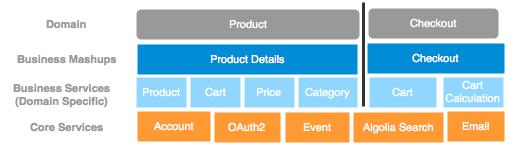
\includegraphics[width=0.8\textwidth]{figures/hybris-architecture-four}
\caption{Microservices Layers}
\label{fig:hybris_architecture/interview/microservices-layers}
\end{center}
\end{figure}
\\
The figure \ref{fig:hybris_architecture/interview/microservices-layers} uncovers only microservices at the backend related to two separate subdomains. The complete architecture covering other domains such as Marketing etc and all layers including User- Interface, \acrshort{PaaS} is shown by figure \ref{fig:hybris_architecture/interview/hybris-architecture}.

\\
\begin{figure}[H]
\begin{center}
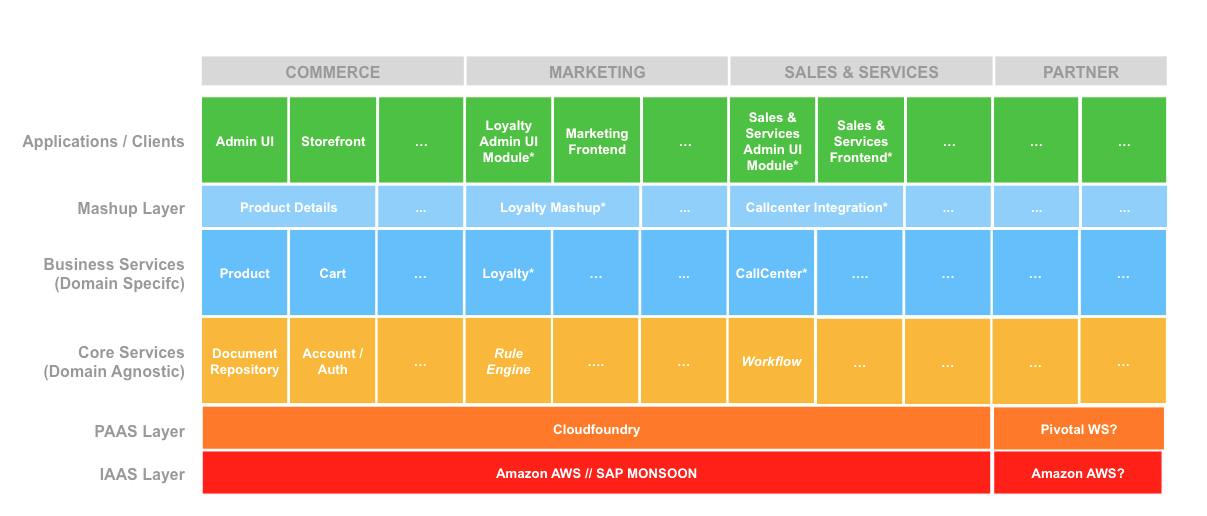
\includegraphics[width=0.9\textwidth]{figures/hybris-architecture-five}
\caption{Hybris Architecture}
\label{fig:hybris_architecture/interview/hybris-architecture}
\end{center}
\end{figure}
\\














